% !TeX program = lualatex
% ================================================================
% Polish Tier 3 Vocabulary Version of ExpandingDoubleBracketsStarter
%
% Generated by the server using the following settings:
%
%   language            Polish (pol)
%   text direction      left to right
%   font                Noto Serif
%   fallback font       Noto Serif
%   built from          latex/starters/targeted/KS3/algebra/expandingDoubleBracketsStarter.tex
%   vocabulary key      latex/starters/targeted/KS3/algebra/expandingDoubleBracketsStarter/L2/pol/expandingDoubleBracketsStarter_polishKey.tex
%   tier 3 vocabulary   green   RGB 0 128 0
%   English text        black   RGB 0 0 0
%   Polish text         purple  RGB 112 48 160
%   layout macros       version 3
%
% Please don't edit any information in this comment block - the server
% compares it against the current settings and rebuilds this file when
% they differ, so changes here would be overwritten. However, feel free
% to make updates to the LaTeX below if you want to edit it.
% ================================================================

\documentclass{beamer}
% ================================================================
% Copied from the English sheet this was translated from, so that
% anything it sets up for itself still works here
% ================================================================
\usetheme{default} % You can swap theme if you like (e.g., Madrid, Boadilla)
\usepackage{tikz} 

% ================================================================
% Answer-overlay helpers
% ================================================================
\newcommand{\ablank}[1]{%
  \alt<2>{\textcolor{red}{#1}}{\underline{\phantom{#1}}}%
}
\newcommand{\ashow}[1]{\uncover<2->{\textcolor{red}{\small #1}}}
\newcommand{\ashowq}[1]{\alt<2->{\textcolor{red}{\small #1}}{?}}

% Answers drawn straight on to a TikZ diagram, revealed on overlay 2 like \ashow.
% Space is reserved on overlay 1, so the diagram does not move between slides.
\usetikzlibrary{overlay-beamer-styles}
\tikzset{
  ans/.style     = {red, thick, visible on=<2->},
  ansfill/.style = {red!15, visible on=<2->},
  anslab/.style  = {red, font=\tiny, visible on=<2->},
}

\title{Starter: Expanding Brackets}
\author{Year 8}
\date{}

% Characters this language's font has not got are borrowed from another,
% rather than being silently dropped - see docs/translated-sheet-latex.md
\directlua{%
  if luaotfload and luaotfload.add_fallback then
    luaotfload.add_fallback("eallatinfallback",
      { "Noto Serif:mode=harf;" })
  else
    tex.error("this luaotfload is too old to register a fallback font")
  end
}
\usepackage[english]{babel}
\babelprovide[import]{polish}
\babelfont[polish]{rm}[Renderer=Harfbuzz, BoldFont={Noto Serif}, ItalicFont={Noto Serif}, BoldItalicFont={Noto Serif}, RawFeature={fallback=eallatinfallback}]{Noto Serif}
\babelfont[polish]{sf}[Renderer=Harfbuzz, BoldFont={Noto Serif}, ItalicFont={Noto Serif}, BoldItalicFont={Noto Serif}, RawFeature={fallback=eallatinfallback}]{Noto Serif}
\newcommand{\ealtext}[1]{\foreignlanguage{polish}{#1}}
\newcommand{\ealtextblock}[1]{{\raggedright\foreignlanguage{polish}{#1}\par}}
% ================================================================
% EAL layout helpers
% ================================================================
\usepackage{xcolor}

\definecolor{ealkeycolour}{RGB}{0,128,0}
\definecolor{ealenglish}{RGB}{0,0,0}
\definecolor{ealtwocolour}{RGB}{112,48,160}

\newsavebox{\ealboxen}
\newsavebox{\ealboxtr}
\newlength{\ealglosswd}
\newlength{\ealglossraise}
\setlength{\ealglossraise}{1.15em}

% a tier 3 word, in English and in translation alike
\newcommand{\ealkey}[1]{\textcolor{ealkeycolour}{#1}}
\newcommand{\ealkeytr}[1]{\textcolor{ealkeycolour}{\ealtext{#1}}}

% One translated word above one English word. Built from kernel
% primitives, never a tabular, which would break wherever the sheet
% loads array, booktabs or tabularx. The box is as wide as the wider of
% the two, so a long translation pushes its neighbours aside instead of
% overlapping them, and it claims its full height so a table row or a
% TikZ node makes room for it.
\newcommand{\ealgloss}[2]{%
  \sbox{\ealboxen}{\ealkey{#1}}%
  \sbox{\ealboxtr}{\small\textcolor{ealtwocolour}{\ealtext{#2}}}%
  \setlength{\ealglosswd}{\wd\ealboxen}%
  \ifdim\wd\ealboxtr>\ealglosswd\setlength{\ealglosswd}{\wd\ealboxtr}\fi
  \leavevmode
  \makebox[\ealglosswd][c]{%
    \makebox[0pt][c]{\usebox{\ealboxen}}%
    \makebox[0pt][c]{\raisebox{\ealglossraise}{\usebox{\ealboxtr}}}%
  }%
}

% opens up line spacing around a block of glosses, so the raised
% translations sit clear of the line above
\newenvironment{ealglossed}{\par\linespread{2.1}\selectfont\ignorespaces}{\par}

% a whole translated sentence above its English counterpart. block level,
% so it does not belong inside a tabular cell
\newcommand{\ealpara}[2]{%
  \par\addvspace{0.5\baselineskip}%
  {\color{ealtwocolour}\ealtextblock{#1}}%
  \penalty200
  {\color{ealenglish}#2\par}%
  \addvspace{0.5\baselineskip}%
}

\begin{document}

\begin{frame}
  \titlepage
\end{frame}

% ---------- STARTER (2x2 layout) ----------
\begin{frame}{Starter: \ealgloss{Expand}{wymnażać nawiasy} each \ealgloss{expression}{wyrażenie}}
\begin{ealglossed}
\begin{minipage}[t]{0.48\textwidth}
  \begin{block}{1) Single \ealgloss{brackets}{nawiasy}}
    \Large \(\;3(y+5)=\ablank{3y+15}\)
  \end{block}
  \vspace{0.5em}
  \begin{block}{3) Double \ealgloss{brackets}{nawiasy}}
    \Large \(\;(x+4)(x-2)=\ablank{x^2+2x-8}\)
  \end{block}
\end{minipage}\hfill
\begin{minipage}[t]{0.48\textwidth}
  \begin{block}{2) Single \ealgloss{brackets}{nawiasy}}
    \Large \(\; a(b-5)=\ablank{ab-5a}\)
  \end{block}
  \vspace{0.5em}
  \begin{block}{4) What is the \ealgloss{area}{pole} of the \ealgloss{rectangle}{prostokąta}?}
    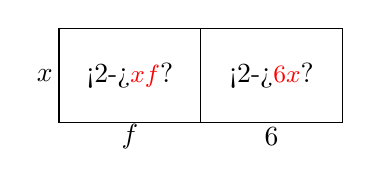
\begin{tikzpicture}[scale=0.6]

% Outer rectangle
\draw (0,0) rectangle (6,2);

% Vertical split
\draw (3,0) -- (3,2);

% Labels for widths
\node at (1.5,-0.3) {$f$};
\node at (4.5,-0.3) {$6$};

% Height label
\node at (-0.3,1) {$x$};

% Area labels
\node at (1.5,1) {\ashowq{$xf$}};
\node at (4.5,1) {\ashowq{$6x$}};

\end{tikzpicture}
    \par\vspace{0.5em}
    \ashow{\ealgloss{Area}{pole} = \(x(f+6)\)}
  \end{block}
\end{minipage}
\end{ealglossed}
\end{frame}

% ---------- ANSWERS ----------
\begin{frame}{Answers}
\begin{ealglossed}
\begin{enumerate}
  \item \(3(y+5)=3y+15\)
  \item \(a(b-5)=ab-5a\)
  \item \((x+4)(x-2)=x^2+2x-8\)
  \item \ealgloss{Area}{pole} = \(xf + 6x = x(f+6)\)
\end{enumerate}
\end{ealglossed}
\end{frame}

% answer macro review note
\begin{frame}
\frametitle{Automated check: answers may need attention}
The answers on these slides may have unresolved formatting issues. An automated
review did not accept them, and rewriting them did not settle it.

The review said the "final answers" frame and the "Answers" frame each show all answers on their first overlay, meaning nothing is hidden until a click. It doesn't name specific slides, only those two frame titles. The two comments are essentially the same complaint repeated, not contradictory, but it's worth checking whether showing all answers immediately is actually a mistake or an intentional design choice.

Please check these slides and either correct them or raise an issue.
\end{frame}

\end{document}